%%%%%%%%%%%%%%%%%%%%%%%%%%%%%%%%%%%%%%%%%%%%%%%%%%%%%%%%%%%%%%%%%%%%%%%%%%%%%%%%
%% Plantilla de memoria en LaTeX para la ETSIT - Universidad Rey Juan Carlos
%%
%% Por Gregorio Robles <grex arroba gsyc.urjc.es>
%%     Grupo de Sistemas y Comunicaciones
%%     Escuela Técnica Superior de Ingenieros de Telecomunicación
%%     Universidad Rey Juan Carlos
%% (muchas ideas tomadas de Internet, colegas del GSyC, antiguos alumnos...
%%  etc. Muchas gracias a todos)
%%
%% La última versión de esta plantilla está siempre disponible en:
%%     https://github.com/gregoriorobles/plantilla-memoria
%%
%% Para obtener PDF, ejecuta en la shell:
%%   make
%% (las imágenes deben ir en PNG o JPG)

%%%%%%%%%%%%%%%%%%%%%%%%%%%%%%%%%%%%%%%%%%%%%%%%%%%%%%%%%%%%%%%%%%%%%%%%%%%%%%%%

\documentclass[a4paper, 12pt]{book}
%\usepackage[T1]{fontenc}

\usepackage[a4paper, left=2.5cm, right=2.5cm, top=3cm, bottom=3cm]{geometry}
\usepackage{times}
\usepackage[utf8]{inputenc}
\usepackage[spanish]{babel} % Comenta esta línea si tu memoria es en inglés
\selectlanguage{spanish}
\usepackage{url}
%\usepackage[dvipdfm]{graphicx}
\usepackage{graphicx}
\usepackage{float}  %% H para posicionar figuras
\usepackage[nottoc, notlot, notlof, notindex]{tocbibind} %% Opciones de índice
\usepackage{latexsym}  %% Logo LaTeX
\usepackage{enumerate} 
\usepackage{verbatim} % comentarios
\usepackage{breakurl}
\PassOptionsToPackage{hyphens}{url}\usepackage{hyperref}
\usepackage{caption}




\title{Memoria del Proyecto}
\author{Nombre del autor}

\renewcommand{\baselinestretch}{1.5}  %% Interlineado

\begin{document}

\renewcommand{\refname}{Bibliografía}  %% Renombrando
\renewcommand{\appendixname}{Apéndice}

%%%%%%%%%%%%%%%%%%%%%%%%%%%%%%%%%%%%%%%%%%%%%%%%%%%%%%%%%%%%%%%%%%%%%%%%%%%%%%%%
% PORTADA

\begin{titlepage}
\begin{center}
\begin{tabular}[c]{c c}
%\includegraphics[bb=0 0 194 352, scale=0.25]{logo} &

\includegraphics[scale=0.25]{img/logo_vect.png} &
\begin{tabular}[b]{l}
\Huge
\textsf{UNIVERSIDAD} \\
\Huge
\textsf{REY JUAN CARLOS} \\
\end{tabular}
\\
\end{tabular}

\vspace{3cm}

\Large
GRADO EN INGENIER\'IA EN SISTEMAS DE TELECOMUNICACI\'ON

\vspace{0.4cm}

\large
Curso Acad\'emico 2018/2019

\vspace{0.8cm}
Trabajo Fin de Grado

\vspace{2.5cm}

\LARGE
GENERADOR DE GR\'AFICOS PARA UN PORTAL LIFERAY UTILIZANDO REACT

\vspace{4cm}

\large
Autor : Rub\'en Barrado Jim\'enez \\
Tutor : Gregorio Robles Mart\'inez
\end{center}
\end{titlepage}

\newpage
\mbox{}
\thispagestyle{empty} % para que no se numere esta pagina


%%%%%%%%%%%%%%%%%%%%%%%%%%%%%%%%%%%%%%%%%%%%%%%%%%%%%%%%%%%%%%%%%%%%%%%%%%%%%%%%
%%%% Para firmar

%%%%%%%%%%%%%%%%%%%%%%%%%%%%%%%%%%%%%%%%%%%%%%%%%%%%%%%%%%%%%%%%%%%%%%%%%%%%%%%%
%%%% Dedicatoria

\chapter*{}
\pagenumbering{Roman} % para comenzar la numeracion de paginas en numeros romanos
\begin{flushright}
\textit{``El éxito es la capacidad de ir de fracaso en fracaso sin perder el entusiasmo''.\\ 
Winston Churchill}
\end{flushright}

%%%%%%%%%%%%%%%%%%%%%%%%%%%%%%%%%%%%%%%%%%%%%%%%%%%%%%%%%%%%%%%%%%%%%%%%%%%%%%%%
%%%% Agradecimientos

\chapter*{Agradecimientos}
%\addcontentsline{toc}{chapter}{Agradecimientos} % si queremos que aparezca en el �ndice
\markboth{AGRADECIMIENTOS}{AGRADECIMIENTOS} % encabezado 

Aquí vienen los agradecimientos\ldots Aunque esta bien acordarse de la pareja, no hay que olvidarse de dar las gracias a tu madre, que aunque a veces no lo parezca disfrutara tanto de tus logros como tu\ldots 
Además, la pareja quizás no sea para siempre, pero tu madre si.

%%%%%%%%%%%%%%%%%%%%%%%%%%%%%%%%%%%%%%%%%%%%%%%%%%%%%%%%%%%%%%%%%%%%%%%%%%%%%%%%
%%%% Resumen

\chapter*{Resumen}
%\addcontentsline{toc}{chapter}{Resumen} % si queremos que aparezca en el �ndice
\markboth{RESUMEN}{RESUMEN} % encabezado
El presente trabajo de fin de grado ha consistido en integrar soluciones de uso extendido en los portales web que suelen ser utilizados por las compañías, empleando el framework de React dentro de la plataforma de Experiencia Digital de Liferay. Para ello se propone la integración de un gestor de contenidos, como es Liferay, con las bibliotecas y funciones de JavaScript, utilizando React.

\vspace{5mm}
Para llevar a cabo la integración, se ha realizado el desarrollo de un portlet o componente, en el cual, a partir de unos datos de entrada, en tiempo real y en formato \textit{JSON}, podamos generar tipos de contenido útil para la web y sus usuarios. En dicho componente podemos ver diferentes datos mostrados en forma de gráficos utilizando bibliotecas que permiten la creación de gráficos con React. Los datos utilizados en este trabajo de fin de grado corresponden al tiempo diario y semanal en las capitales de las comunidades autónomas de España.

\vspace{5mm}
Este proyecto se ha llevado a cabo en colaboración con la empresa \textit{Everis}, para poder solucionar los inconvenientes causados al intentar implementar funciones JavaScript en sus proyectos realizados con Liferay.




% Aqui viene un resumen del proyecto. Ha de constar de tres o cuatro parrafos, donde se presente de manera clara y concisa de que va el proyecto. 
% Han de quedar respondidas las siguientes preguntas:

% \begin{itemize}
%   \item De que va este proyecto? Cual es su objetivo principal?
%   \item Cmo se ha realizado? Qu tecnologas estn involucradas?
%   \item En qtexto se ha realizado el proyecto? royecto
% dentro de un marco general?
% \end{itemize}

% Lo mejor es escribir el resumen al final.

%%%%%%%%%%%%%%%%%%%%%%%%%%%%%%%%%%%%%%%%%%%%%%%%%%%%%%%%%%%%%%%%%%%%%%%%%%%%%%%%
%%%% Resumen en inglés

\chapter*{Summary}
%\addcontentsline{toc}{chapter}{Summary} % si queremos que aparezca en el índice
\markboth{SUMMARY}{SUMMARY} % encabezado
This final project has consisted of integrating solutions of extended use in web portals that are usually used by companies using the React framework within Liferay's Digital Experience platform. For this purpose, it is proposed to integrate a content management system, such as Liferay, with the JavaScript libraries and functions, using React.

\vspace{5mm}
To carry out the integration, I have developed a portlet or component, in which, from some input data, in real time and in JSON format, we can generate types of content useful for the web and its users. In this component we can see the data displayed by graphs using libraries that allow the creation of graphics with React. The data used in this final project correspond to daily and weekly weather in the capitals of the Spanish regions.

\vspace{5mm}
This project has been carried out in collaboration with the company Everis, in order to solve the inconveniences caused when trying to implement JavaScript functions in their projects made with Liferay.



% Here comes a translation of the ``Resumen'' into English. Please, double check it for correct grammar and spelling.
% As it is the translation of the ``Resumen'', which is supposed to be written at the end, this as well should be filled out
% just before submitting.


%%%%%%%%%%%%%%%%%%%%%%%%%%%%%%%%%%%%%%%%%%%%%%%%%%%%%%%%%%%%%%%%%%%%%%%%%%%%%%%%
%%%%%%%%%%%%%%%%%%%%%%%%%%%%%%%%%%%%%%%%%%%%%%%%%%%%%%%%%%%%%%%%%%%%%%%%%%%%%%%%
% �NDICES %
%%%%%%%%%%%%%%%%%%%%%%%%%%%%%%%%%%%%%%%%%%%%%%%%%%%%%%%%%%%%%%%%%%%%%%%%%%%%%%%%

% Las buenas noticias es que los �ndices se generan autom�ticamente.
% Lo �nico que tienes que hacer es elegir cu�les quieren que se generen,
% y comentar/descomentar esa instrucci�n de LaTeX.

%%%% �ndice de contenidos
\tableofcontents 
%%%% �ndice de figuras
\cleardoublepage
%\addcontentsline{toc}{chapter}{Lista de figuras} % para que aparezca en el indice de contenidos
\listoffigures % indice de figuras
%%%% �ndice de tablas
%\cleardoublepage



%%%%%%%%%%%%%%%%%%%%%%%%%%%%%%%%%%%%%%%%%%%%%%%%%%%%%%%%%%%%%%%%%%%%%%%%%%%%%%%%
%%%%%%%%%%%%%%%%%%%%%%%%%%%%%%%%%%%%%%%%%%%%%%%%%%%%%%%%%%%%%%%%%%%%%%%%%%%%%%%%
% INTRODUCCI�N %
%%%%%%%%%%%%%%%%%%%%%%%%%%%%%%%%%%%%%%%%%%%%%%%%%%%%%%%%%%%%%%%%%%%%%%%%%%%%%%%%

\cleardoublepage
\chapter{Introducci\'on}
\label{sec:intro} % etiqueta para poder referenciar luego en el texto con ~\ref{sec:intro}
\pagenumbering{arabic} % para empezar la numeraci�n de p�gina con n�meros

Este Trabajo Fin de Grado tiene como principal objetivo la integración de bibliotecas de JavaScript, en este caso, React, en un gestor de contenidos, llamado Liferay para poder implementar páginas web con las características de ambas tecnologías. En este proyecto se ha realizado la integración mediante la generación de gráficos utilizando las bibliotecas “Chart.js”, “React-chartjs-2” y “React-chartjs2”, de React.


\section{Contexto}
\label{sec:contexto}
Actualmente son muchas las empresas que se han decantado por usar gestores de contenidos para realizar sus páginas web propias o las de sus clientes. Esto es debido a que los gestores de contenidos Open Source son capaces de facilitar el trabajo y poder llevar a cabo páginas web que pueden ser controladas por personas que no tienen conocimientos informáticos.

\vspace{5mm} %5mm vertical space
Los gestores de contenidos permiten la creación, manipulación y publicación de contenidos en una página web de manera muy sencilla y personalizable. Se pueden implementar nuevas funcionalidades una vez la web está operativa para los usuarios sin la necesidad de intervención de un desarrollador.

\vspace{5mm} %5mm vertical space
La mayoría de las compañías emplean estos gestores de contenidos para crear la Intranet de usuarios de sus clientes debido a que proporciona ayuda a la hora de desarrollar soluciones empresariales, con resultados inmediatos y a largo plazo, ofreciendo un framework de desarrollo capaz de adaptarse a las necesidades requeridas.

\vspace{5mm} %5mm vertical space
El principal inconveniente de emplear este método para la creación de una Intranet es que el código fuente es más complejo que emplear un desarrollo a medida para dicha página. Este inconveniente lo podemos evitar implantando JavaScript y sus librerías en el gestor de contenidos. 

\vspace{5mm} %5mm vertical space
En un gestor de contenidos cada página del portal actúa como un contenedor de diferentes aplicaciones, y si, por ejemplo, en una página web hay varias subpáginas se podría usar el mismo contenido en todas ellas si fuera necesario,  además de poder eliminarlo de una subpágina en un momento dado o cambiarlo de lugar. De este modo, al tener integrado React con el gestor de contenidos, se puede añadir la web creada con React en cualquier parte de nuestro portal, incluso se podría tener la web en diferentes subpáginas sin necesidad de repetir el código.

\vspace{5mm} %5mm vertical space
Los portlets con React o con JavaScript se pueden desplegar en Liferay por otros medios, como desplegarlos en otras plataformas y accediendo a ellos vía \textit{API}\footnote{Application Programming Interface}, pero este método es más rápido y más sencillo de realizar debido a que desplegamos el portlet directamente, pudiendo ir probando nuestros cambios en React según vamos diseñando el componente.


\section{Motivaci\'on}
\label{sec:motivacion}
Este proyecto ha sido realizado en colaboración con la empresa \textit{Everis}\footnote{\url{https://www.everis.com/spain/es/home-1}}, en la que estoy trabajando actualmente. En dicha empresa, he trabajado en varios proyectos llevados a cabo por el gestor de contenidos de Liferay, muy utilizado en el mundo empresarial como base de portales públicos y privados, tales como intranets o portales de cliente. Por norma general, todos los componentes desarrollados sobre la tecnología Liferay se desarrollan en Java.

\vspace{5mm} %5mm vertical space
La integración de React en Liferay era un trabajo pendiente de hacer que podría incluir grandes mejoras en los proyectos con las que trabaja la empresa, por lo que ha sido una gran oportunidad de aprendizaje en dicha empresa. React es una de las más populares bibliotecas de JavaScript. En portales de Liferay, React sería muy importante a la hora de crear componentes debido a la velocidad y fluidez de las peticiones bajo demanda. Estos componentes son reutilizables en todo tipo de portales y proyectos desarrollados por Liferay, lo que es una gran ventaja.

\vspace{5mm} %5mm vertical space
React es una de las plataformas más utilizadas por las empresas, por encima de \textit{Angular}, que hasta hace poco dominaba el mercado por encima de React, por lo que muchas empresas piden desarrollos llevados a cabo con React, por lo que era una buena oportunidad para incorporar esta librería de JavaScript en la plataforma Liferay.

\vspace{5mm} %5mm vertical space
Como hemos visto, React es un framework que está ganando terreno y está incrementando su uso en el mercado, tal y como podemos ver en la Figura~\ref{fig:react_mercado}, en la cual podemos ver la comparativa, realizada por Jobfluent\footnote{\url{https://www.jobfluent.com/es}}, entre las librerías de React, Angular y VUE, donde podemos ver el crecimiento de React respecto al resto de frameworks.
\begin{figure}[h]
  \centering
  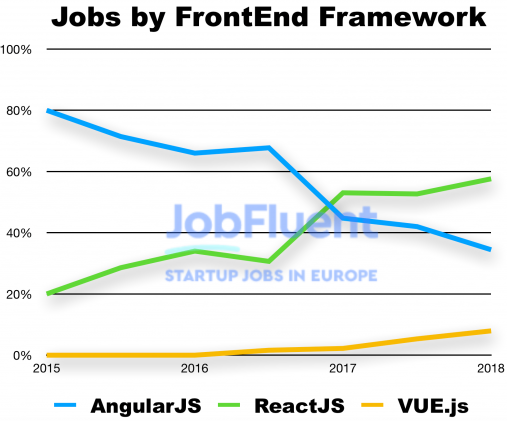
\includegraphics{img_usadas/react_mercado.png}
  \caption{Comparativa entre las librerías más populares de JavaScript en el mercado}
  \label{fig:react_mercado}
\end{figure}

\vspace{5mm}
Por tanto, la implementación de este proyecto plantea como principal reto la utilización de dos tecnologías extendidas en el mercado y que habitualmente no se utilizan de forma conjunta, por un lado cubre las necesidades de las empresas que apuestan por gestores de portales como Liferay, y otro responde a la implantación de React como tecnología asentada en el mercado y en constante evolución.


\section{Estructura de la memoria}
\label{sec:estructura}
En este apartado se va a describir la estructura de la memoria, que se ha dividido en 6 capítulos explicados a continuación:


\begin{enumerate}
    \item \emph{Introducción}
    
    En este primer capítulo se explica el contexto en el que se ha desarrollado, su motivación y la estructura de la memoria.
    
    \item \emph{Objetivos}
    
    En este apartado se detallan los objetivos del proyecto.
    
    \item \emph{Estado del arte}
    
    En este capítulo se explica el estado del arte de las tecnologías utilizadas en este trabajo. 
    
    \item \emph{Instalación e implementación}
    
    Donde se explican los pasos necesarios para la instalación del entorno en el que se ha desarrollado el proyecto, así como su implementación.

       \item \emph{Resultados obtenidos}
    
    En este apartado se muestran los resultados obtenidos.
    
        \item \emph{Conclusiones}
    
    Por último, se detallan las conclusiones tras la consecución de los objetivos.
    
 \end{enumerate}

%%%%%%%%%%%%%%%%%%%%%%%%%%%%%%%%%%%%%%%%%%%%%%%%%%%%%%%%%%%%%%%%%%%%%%%%%%%%%%%%
%%%%%%%%%%%%%%%%%%%%%%%%%%%%%%%%%%%%%%%%%%%%%%%%%%%%%%%%%%%%%%%%%%%%%%%%%%%%%%%%
% OBJETIVOS %
%%%%%%%%%%%%%%%%%%%%%%%%%%%%%%%%%%%%%%%%%%%%%%%%%%%%%%%%%%%%%%%%%%%%%%%%%%%%%%%%

\cleardoublepage % empezamos en página impar
\chapter{Objetivos} % título del capítulo (se muestra)
\label{chap:objetivos} % identificador del capítulo (no se muestra, es para poder referenciarlo)

\section{Objetivo general} % título de sección (se muestra)
\label{sec:objetivo-general} % identificador de sección (no se muestra, es para poder referenciarla)

El objetivo principal de este proyecto ha sido poder integrar Liferay con el framework de React, pudiendo utilizar sus bibliotecas y funciones. Para ello ha sido necesario poder conocer Liferay y su funcionamiento respecto a módulos o portlets pudiendo configurar sus dependencias. Estas dependencias son esenciales a la hora de conectar el gestor de contenidos con React, debido a que al ser una biblioteca de JavaScript no es posible su utilización dentro de Liferay.

La utilización sólo es posible a partir de la versión 7.1 de Liferay, en la cual tenemos un plugin que permite la integración. Hay varias formas de realizar dicha integración:
\begin{itemize}
    \item Configurando las dependencias a mano y modificando los ficheros necesarios para poder conectar React.
    \item Con una serie de comandos \textit{npm}\footnote{\url{https://www.npmjs.com}} en los cuales se configuran las dependencias automáticamente.
\end{itemize}

En este caso hemos optado por la segunda opción debido a que es más rápida de configurar y más asequible, aunque sea necesario realizar varios pasos para la instalación de todos los paquetes necesarios, dicha instalación se explicará en el capítulo~\ref{sec:estado-del-arte}.

\section{Objetivos secundarios}
\label{sec:objetivos-secundarios}
En el camino hasta conseguir el objetivo principal, ha sido necesario tener que comenzar a formarme con la librería React y con el gestor Liferay. Este aprendizaje me ha resultado interesante debido a dos razones:

\begin{enumerate}
    \item La formación con Liferay debido a la posibilidad que te ofrece empresarialmente tener conocimientos sobre este gestor, ya que es altamente utilizado por las empresas de este sector.
    \item La formación con JavaScript, y en especial con la librería React, debido a que últimamente está siendo muy demandado por las empresas y muy utilizado en el mercado.
    
\end{enumerate}

Otro de los objetivos a la hora de realizar este proyecto era poder familiarizarme con las dos tecnologías debido a que en muchos proyectos utilizar ambas tecnologías sería de gran ayuda.

%%%%%%%%%%%%%%%%%%%%%%%%%%%%%%%%%%%%%%%%%%%%%%%%%%%%%%%%%%%%%%%%%%%%%%%%%%%%%%%%
%%%%%%%%%%%%%%%%%%%%%%%%%%%%%%%%%%%%%%%%%%%%%%%%%%%%%%%%%%%%%%%%%%%%%%%%%%%%%%%%
% TECNOLOGÍAS UTILIZADAS %
%%%%%%%%%%%%%%%%%%%%%%%%%%%%%%%%%%%%%%%%%%%%%%%%%%%%%%%%%%%%%%%%%%%%%%%%%%%%%%%%

\chapter{Estado del arte} 
\label{sec:estado-del-arte}
En este apartado se va a hablar de las tecnologías utilizadas para la realización de este proyecto. Dichas tecnologías son Liferay, React y JSON\footnote{JavaScript Object Notation}.

Para poder hablar de Liferay, primero debemos tener unos conceptos claros sobre el significado de un gestor de contenidos.

\section{Gestor de contenidos}
\label{subsec:gestor-de-contenidos}
Un gestor de contenidos o \emph{CMS} (Content Management System) es una aplicación a la que accedemos a través de un navegador que permite crear, manipular y organizar contenidos dentro de una página web sin ser necesario tener conocimientos informáticos. Estos contenidos son administrados por los usuarios con roles determinados dentro de la página web ~\cite{cms_tech}.


\vspace{5mm}
Los pasos que hay que seguir para tener un contenido web son: 
\begin{enumerate}
    \item \emph{Creación del contenido web}: generado por editores integrados en los que se diseña el contenido como necesite el usuario.
    \item \emph{Publicación del contenido web}: una vez se ha creado el contenido web podremos publicarlo y tenerlo disponible para usarlo.
    \item \emph{Gestión del contenido web}: una vez publicado el contenido estará disponible para usarlo en la zona de la web que queramos, pudiéndolo cambiar de lugar, editarlo o eliminarlo. Los contenidos puedes ser organizados en varias páginas.
    \item \emph{Presentación del contenido web}: podremos ver su resultado final desde cualquier navegador.
\end{enumerate}

\vspace{5mm}
Un \emph{CMS} tiene varias características~\cite{cms_misc}:
\begin{itemize}
    \item Proceso de creación de contenido rápido, intuitivo, dinámico y fácil, donde no es necesario tener conocimientos informáticos.
    \item Gran flexibilidad, velocidad, rendimiento y seguridad de la web.
    \item Posee medios de soporte a los usuarios y administración del sitio sencilla.
    \item Reducción en los costes de mantenimiento.
    \item Gestión de las subpáginas que puede haber en una web y el multilenguaje.
    \item Soporte en varios dispositivos y canales.
\end{itemize}

\vspace{5mm}
Aparte, debe cumplir varias funciones para poder ofrecer contenidos de alto nivel que son: 
\begin{itemize}
    \item Herramientas que permitan crear contenidos como plantillas, estructuras y workflows.
    \item Interoperabilidad con otras tecnologías para poder obtener un mejor resultado.
    \item Capacidad de personalización en todos los contenidos.
    \item Integración con los sistemas de entrega.
\end{itemize}

\vspace{5mm}
Los gestores de contenidos pueden ser de diferentes sistemas, para el caso de Liferay es un sistema de Experiencia Digital \textit{DXP}\footnote{Digital Experience Platform}. La principal función de un sistema \textit{DXP} es la de proporcionar un contenido adaptable a cualquier canal digital en la creación del contenidos, además de mejorar las capacidades de negocio por medio de la digitalización. Últimamente, todos los \textit{CMS} se están convirtiendo en \textit{DXPs} debido a que las necesidades de las empresas son digitales y con \textit{DXP} se pueden aprovechar las experiencias de los clientes de un \textit{CMS} y añadirla a las capacidades de integración.


\section{Liferay}
\label{subsec:liferay}
Este Trabajo Fin de Grado es un proyecto de Software Libre, lo que significa que es un programa que ofrece una serie de libertades a la hora de modificar el código, estudiarlo y utilizarlo en cualquier sitio y para cualquier propósito.

Al ser un proyecto desarrollado con Liferay, debe cumplir las libertades que ofrece un Software Libre. Esto implica que se permite el acceso y la modificación del código para el beneficio de su comunidad.


\vspace{5mm}
Liferay es un portal de gestión de contenidos Open Source basado en Java EE orientado a la solución y creación de portales web empresariales con resultados inmediatos y a largo plazo. Se basa en una arquitectura modular que proporciona herramientas de desarrollo. Se trata de reutilizar marcos y bibliotecas, a la vez que permite crear los propios~\cite{liferay_dev}.


\vspace{5mm}
Liferay puede utilizarse con la mayoría de servidores de aplicaciones, contenedores de servlets (en nuestro caso Tomcat) y base de datos (\textit{MySQL}, \textit{Oracle}).

\vspace{5mm}
En Liferay hay una comunidad con un foro, donde los usuarios exponen sus dudas para ser resueltas. Las características de Liferay son: 
\begin{itemize}
    \item Facilitar la creación, gestión y administración de portales web, con la colaboración de sus usuarios.
    \item Cada página del portal actúa como un contenedor de diferentes portlets, que puede ser una línea de texto o, como en el caso de este trabajo, una aplicación capaz de obtener datos en tiempo real de una \textit{API} y mostrarlos en forma de gráficos. 
    \item Estabilidad para garantizar la calidad de la aplicación.
    \item Seguridad.
    \item Eficiencia y rendimiento.
    \item Escalabilidad y durabilidad.
    \item Portabilidad, usabilidad y configurabilidad.
\end{itemize}

\vspace{5mm}
Puede utilizarse para~\cite{liferay_dev_tutorials}:
\begin{itemize}
\item Desarrollar aplicaciones completas (portlets o módulos).
\item Personalizar una aplicación.
\item Crear nuevos servicios web para usarlo con un sistema externo, como por ejemplo un móvil.
\item Desarrollar aplicaciones móviles con Liferay Screens.
\item Desarrollar temas de apariencia personalizados.
\end{itemize}

Todas estas utilidades se desarrollan como módulos en archivo \textit{JAR}\footnote{Java ARchive} que siguen estándares \textit{OSGi}\footnote{Open Services Gateway initiative}, que es un framework usado para desarrollar aplicaciones Java, que mantienen los plugins en sistemas \textit{WAR}\footnote{Web Application Archive}.

\vspace{5mm}
Un módulo o portlet, es un componente que puede usarse para crear aplicaciones de gran nivel mezclándose entre ellos y combinándose. Liferay es usado para desplegar los módulos y así crear un portal con varios contenidos web.

Un portal es una plataforma donde se construyen aplicaciones y sitios web, con Liferay podremos tener un portal con múltiples características en los que podemos desarrollar gran variedad de aplicaciones gestionando sus usuarios, creando varios sitios o páginas que necesitan poco mantenimiento, y creando entornos colaborativos.

Los portales se dividen en sitios compuestos por páginas donde se muestran los contenidos (portlets). Liferay puede asignar roles a determinados usuarios o grupos de usuarios que pueden modificar los contenidos, eliminarlos, crearlos y organizarlos. Estos usuarios tienen una serie de contenidos y funcionalidades que les aporta Liferay por defecto, que son:

\begin{itemize}
\item Gestión de contenidos (visor de contenido web, publicador de contenidos, galería multimedia, documentos y multimedia, aplicaciones anidadas).
\item Menú de navegación.
\item Búsqueda (barra de búsqueda, opciones de búsqueda, sugerencias, resultados).
\item Colaboración (blogs, calendarios, formularios, foros).
\item Comunidad (comentarios, sitios web, valoraciones, notificaciones).
\item Herramientas (búsqueda web, login, selector de idioma).
\item Noticias (alarmas, avisos, redes sociales).
\item Social (actividades, contactos, miembros, perfil).
\item Wiki (visor de la wiki, wiki, menú de árbol de la wiki).
\end{itemize}

Todos estos tipos de contenidos pueden ser usados por los usuarios sin necesidad de realizar ningún desarrollo informático, simplemente debe estar creado el contenido del tipo que queramos usar y moverlo a la zona del portal que deseemos. 

Si fuera preciso, como en el caso de este proyecto, de crear algún tipo de contenido que no tenemos por defecto, podremos crear portlets y gestionarlos.

\vspace{5mm}
Liferay es un gestor de contenidos que permite instalar y gestionar portlets. Estos portlets pueden ser movidos a cualquier página creada en el portal, pudiendo introducir todos los portlets que queramos en cada página, como ocurre con los contenidos que tiene Liferay por defecto.

Es una plataforma que ofrece crear aplicaciones web, móviles y servicios rápidamente. Una de las características de Liferay es la versatilidad para crear todo tipo de sitios web como intranets, entornos colaborativos y aplicaciones móviles. Se puede implementar con contenedores de \textit{JavaEE}\footnote{Java Enterprise Edition} y otros servidores admitiendo una gran variedad de base de datos sin necesidad de cambiar el código fuente.

Este gestor de contenidos es Open Source, o código abierto, que sigue un modelo de desarrollo colaborativo y, además, se basa en los estándares, lo que hace reducir el bloqueo en Liferay. 

\vspace{5mm}
Para la realización de este proyecto es necesario tener una versión de Liferay 7.1 o superior, debido a que es la versión que soporta el estándar JavaScript, gracias a \textit{Babel}\footnote{\url{https://babeljs.io/}} y a un plugin que se puede instalar en el \textit{MarketPlace}\footnote{\url{https://web.liferay.com/es/marketplace}} de Liferay, llamado \textit{Liferay JS Portlet Extender}\footnote{url{https://web.liferay.com/es/marketplace/-/mp/application/115543020}}. Este plugin está disponible a partir de la versión 7.1, y se activa a través de \textit{Marketplace} en el panel de control de Liferay, por lo que en las versiones anteriores no se podía usar el estándar JavaScript. Además de éste, Liferay soporta varios estándares importantes~\cite{liferay_dxp}:

\begin{itemize}
\item Portlets 1.0 y Portlets 2.0 (JRS-168 y JRS-286): permite la ejecución de cualquier portlet.
\item JSF (JRS-127, JRS-314 y JRS-344): permite crear aplicaciones web basadas en componentes.
\item EcmaScript 2015: permite el estándar JavaScript. Este estándar es el que nos permite realizar el proyecto.
\item Servicio de interoperabilidad de gestión de contenido (CMIS): permite que los documentos de Liferay se comporten como una interfaz con cualquier repositorio externo.
\item Repositorio de contenido Java (JSR-170).
\item JAX-RS y JAX-WS: permite la creación de servicios web.
\end{itemize}

\vspace{5mm}
Liferay se basa en varias tecnologías importantes~\cite{liferay_dev_tutorials}:

\begin{itemize}
\item Para Front-end utiliza\textit{ Metal.js}, \textit{Bootstrap} y \textit{Sass}.
\item Para Mobile utiliza Liferay Screen, Android e iOS.
\item Para Back-end utiliza \textit{OSGI}, \textit{Spring} (para transacciones), \textit{JavaEE}, \textit{Hibernate} (acceso a la base de datos), \textit{Ehcache} (almacenamiento en la caché) y \textit{Elasticsearch} (para búsqueda).
\end{itemize}

\vspace{5mm}
El gestor de contenidos Liferay tiene una arquitectura que debe cumplir que el producto sea utilizable, rápido, robusto y personalizable. La arquitectura de Liferay es modular, como se ha dicho anteriormente, esto hace que los módulos cumplan con sus definiciones, implementaciones, prioridades y dependencias.

Al tener una arquitectura modular y basada en componentes, al tener un problema, en vez de cambiar la aplicación entera para arreglarlo, en el caso de tener una arquitectura monolítica, simplemente deberíamos modificar el módulo que está teniendo problemas para solucionar el error, permitiendo además, poder volver al inicio en el caso de no ser necesaria ninguna modificación.

Una aplicación basada en componentes ayuda al desarrollador en:
\begin{itemize}
\item Poder escribir la aplicación en paralelo con otros desarrolladores que realizan un componente diferente.
\item Poder extender la aplicación creando nuevos componentes.
\item Poder habilitar y deshabilitar los componentes.
\end{itemize}

\vspace{5mm}
El tipo de web más utilizado con Liferay es la creación de Intranets, ya que ofrece una gran capacidad de comunicación personalizada para cada usuario, debido a~\cite{liferay_intranets}:

\begin{itemize}
\item Workflows personalizados.
\item Experiencia de usuario moderna.
\item Gestión de activos digitales.
\item Contenidos modificables por usuarios dependiendo de su rol.
\item Integración con sistemas existentes utilizando Liferay DXP.
\item Capacidad de crear un entorno móvil.
\item Unifica los sitios corporativos de los usuarios mediante un login.
\end{itemize}



\vspace{5mm}
\subsection{MVC}
\label{subsec:mvc}
Las aplicaciones web se suelen desarrollar siguiendo un patrón. El patrón que sigue Liferay es el Modelo Vista Controlador (MVC), cuyas características son~\cite{liferay_dev_tutorials}:
\begin{itemize}
\item Mejorar la escalabilidad.
\item Facilitar el mantenimiento.
\item Promover la reutilización.
\end{itemize}

El patrón MVC se divide en:
\begin{itemize}
\item Modelo: contiene los datos de la aplicación y la lógica para usarlos.
\item Vista: se encarga de la presentación de los datos.
\item Controlador: se encarga de controlar los datos entre la vista y el modelo. Gestiona lo lógica de la aplicación actuando de intermediario entre modelo y vista.
\end{itemize}

\vspace{5mm}
El MVC es usado por la gran mayoría de las aplicaciones web, pero Liferay ha desarrollado su propio MVC, que se diferencia en:

\begin{itemize}
\item Ser más ligero.
\item No tiene la necesidad de mantener los archivos sincronizados.
\item Evita escribir código repetido.
\item Oculta la complejidad de los portlets y facilita las operaciones comunes.
\end{itemize}


\subsection{Portlet}
\label{subsec:portlet}
Una vez hemos introducido Liferay, es necesario conocer el concepto de portlet, que es lo que se ha desarrollado en este trabajo. Un portlet es un componente modular reutilizable de un portal web. Liferay es un contenedor de portlets que permite la creación, utilización y eliminación de cada uno de ellos, pudiendo ser utilizados en cualquier portal. Sus características son~\cite{portlet_ibm}: 

\begin{itemize}
\item Generan contenido dinámicamente.
\item Interactúan con el portal mediante peticiones y respuestas.
\item Tiene un ciclo de vida controlado por el contenedor.
\item Son gestionados por el contenedor.
\item No pueden generar contenido arbitrario.
\item El contenedor procesa sus solicitudes.
\end{itemize}

Al interactuar con el portal en las peticiones y las respuestas, el portlet en las respuestas devuelve contenido que es mostrado en los navegadores. La diferencia entre un portlet y otros tipos de navegadores web es que los portlets se ejecutan en una parte de la página web, esto hace que el resto de la página este controlado por otros componentes. 

Se colocan en las páginas por los usuarios que tienen los roles correspondientes o los administradores. Como se ha dicho anteriormente, en una página puede haber muchos portlets diferentes, pudiendo cambiar su colocación y su diseño en cualquier momento. En una página se pueden configurar diferentes portlets y a cada uno le podemos poner el tamaño que queramos, dependiendo de la configuración que tenga la página en la que se coloquen.

\vspace{5mm}
Al igual que Liferay, los portlets están basados en estándares, y además de los estándares de Liferay de Portlets 1.0 y 2.0, recientemente se ha lanzado el Portlet 3.0 que permite la evolución del portlet y su portal.

Los portlets manejan solicitudes en diferentes fases. Sus fases son~\cite{portlet_liferay}:
\begin{itemize}
\item Render: Genera el contenido del portlet. Si se ejecuta esta fase en un portlet, también lo hace con el resto de portlets en la página. Esta fase se vuelve a generar cuando se completa la fase Action y Event.
\item Action: Cuando se genera una acción, se actualiza el estado del portlet
\item Event: Procesa los eventos generados en la fase Action.
\item Resource-serving: Sirve un recurso independiente del ciclo de vida, lo que permite a un portlet ser dinámico sin necesidad de ejecutar las fases anteriores. En esta fase se manejan las solicitudes \textit{AJAX}.
\end{itemize}


Los portlets tienen, además, diferentes modos que indican la función que se está realizando en él:
\begin{itemize}
\item Modo de visualización: es el modo que permite acceder a la funcionalidad principal del portlet.
\item Modo de edición: es el modo de configuración del portlet, permite personalizar el portlet.
\item Modo de ayuda: es el modo que muestra la información de ayuda del portlet.
\end{itemize}



\section{JavaScript}
\label{subsec:javascript}
Para poder hablar de React, framework sobre el que está desarrollado el proyecto, es necesario saber unos conocimientos básicos de JavaScript. Es un lenguaje de programación, que está presente en muchos navegadores web, introducido en el año 1995 como una forma de añadir programas a una página web en el navegador \textit{Netscape} \textit{Navigator}. Desde entonces es un lenguaje muy utilizado, usado en el 90\% de páginas web, que hace posible aplicaciones web modernas y dinámicas~\cite{js_book}.

\vspace{5mm}
A pesar de su nombre, JavaScript no tiene nada que ver con el lenguaje de programación Java, el nombre se debe a una estrategia de marketing debido a la importancia del lenguaje Java en esos momentos. Es un lenguaje de programación que no necesita ser compilado para probar su funcionamiento, simplemente se puede probar el código en el navegador directamente. JavaScript sigue el estándar \textit{ECMAScript} para que sea independiente de cualquier empresa.

\vspace{5mm}
Las características de JavaScript son:

\begin{itemize}
\item Es un lenguaje relativamente fácil de aprender.
\item Desarrollado por Netscape.
\item Funciona en diferentes dispositivos y navegadores.
\item Es un lenguaje rápido y ligero.
\end{itemize}

Es soportado por todos los navegadores, a partir de la versión \textit{ECMAScript} \textit{2015}, y actualmente nos encontramos en la versión \textit{ECMAScript} \textit{2016}.



\section{React}
\label{subsec:react}
Este proyecto de fin de carrera está basado principalmente en conectar las tecnologías de Liferay y de React, para conseguir tener un portlet programado con el lenguaje de React en Liferay.

\vspace{5mm}
React es una de las librerías de JavaScript que permite manejar de forma eficiente la interfaz de usuario de las aplicaciones web. Su desarrollador fue \textit{Facebook} y fue creado para resolver las propias necesidades de la compañía con el mantenimiento del código de los anuncios. Actualmente sigue siendo utilizado en \textit{Facebook} para darle soporte a la página, así como realizar actualizaciones de forma permanente~\cite{react_misc}.

\vspace{5mm}
Sus principales ventajas son:

\begin{itemize}
\item Su gran ecosistema: Es una de las librerías con mayor trayectoria, se generaron muchas librerías extendiendo sus características y potencialidades, permitiendo realizar todo tipo de programas que nos propongamos.
\item Su estabilidad y alta compatibilidad: Es una librería que hace evolucionar todas sus versiones y sus librerías que hace que no existan quiebres de compatibilidad entre ellas generando una gran estabilidad.
\item Su performance: Es una librería liviana que genera tiempos de carga inicial muy rápidos. Además, la actualización de pantalla es muy rápida, lo que permite renderizaciones parciales e inteligentes mediante su Virtual Dom y el proceso de reconciliación.
\end{itemize}

Debido a estos motivos React es muy sólida y fundamentada. Representa, a nivel de arquitectura en el patrón MVC, la V del modo Vista, lo que hace que se pueda combinar con otras librerías de JavaScript~\cite{react_book}.

\vspace{5mm}
React es una librería de código abierto, declarativa, eficiente y flexible que permite construir interfaces de usuario, componentes interactivos y reutilizables, con el objetivo de facilitar el desarrollo de \textit{SPA}\footnote{Single Page Applications}, obteniendo un gran rendimiento. Es una librería que está mantenida por desarrolladores de \textit{Facebook} e \textit{Instagram}, al igual que por desarrolladores independientes. Los componentes interactivos se crean de forma sencilla diseñando vistas simples para cada usuario en la aplicación que hacen que tu código sea más predecible y más fácil de depurar. 

\vspace{5mm}
El nacimiento de React comienza en 2011 cuando Pete Hunt y unos desarrolladores de \textit{Facebook} crean un port de \textit{XHP} en una aplicación \textit{SPA}. Este tipo de aplicación requiere un gran número de peticiones al servidor que \textit{XHP} no conseguía resolver, por lo que los desarrolladores solicitaron usar \textit{XHP} en el navegador con JavaScript, dando lugar a ReactJS.

\vspace{5mm}
Otras librerías parecidas a React son \textit{Meteor} y \textit{Angular}, que permiten que se actualice de forma automática la interfaz de usuario cuando los datos de la aplicación cambian. La diferencia entre estas librerías y React es la forma en la que se programa con React, debido a que se utiliza una programación orientada a videojuegos, mientras que el resto se realiza una programación orientada al sistema \textit{“data-binding”}. Esta diferencia hace que con React tengamos una renderización parcial inmediata, mientras que el resto tiene una renderización persistente. 

Al tener una renderización parcial e inmediata, se renderiza todo con cada cambio que se haga en el código de forma automática, por lo que React es capaz de autogestionarse. Esto se realiza mediante su Virtual Dom, donde está contenido la estructura de datos, el sistema de eventos sintéticos y el gestor de memoria. Con cada cambio en un componente de React, los pasos que se realizan son los siguientes~\cite{react_book}:

\begin{enumerate}
\item Se genera un nuevo árbol Virtual Dom.
\item Se compara con el Virtual Dom previo.
\item Se deciden cuáles son los cambios mínimos a realizar.
\item Se mandan los cambios a la cola.
\item Se procesan los cambios en el navegador.
\end{enumerate}

\vspace{5mm}
En el Virtual Dom tenemos el sistema de eventos sintéticos, que quiere decir que React tiene su propio sistema de eventos que crea un único manejador de evento nativo en el nivel superior de la estructura de cada componente, por lo que no es necesario utilizar otras librerías como \textit{jQuery}\footnote{\url{https://jquery.com/}}, lo que hace que tengamos menos código que desarrollar. El sistema está normalizado por lo que es operable en todos los navegadores, además, es capaz de diferenciar entre eventos “\textit{desktop}” (click con el ratón) y eventos móviles (táctil de la pantalla). 

\vspace{5mm}
React ayuda a los desarrolladores a crear aplicaciones web que utilizan un gran intercambio de datos, preocupándose solamente de la interfaz de usuario de la aplicación. El código programado en React se realiza a través de componentes, que se renderizan automáticamente, como se ha comentado anteriormente. Una interfaz de usuario es creada a partir de componentes, que encapsulan el funcionamiento y la presentación. Los componentes se basan en otros componentes para solucionar las necesidades más complejas. Al estar basado en componentes, se pueden pasar datos a través de la aplicación sin modificar el estado fuera del DOM.

\vspace{5mm}
Otra característica de React es que es isomórfico, que quiere decir que con un mismo código se puede renderizar tanto en cliente como en el servidor disminuyendo la carga de trabajo para realizar aplicaciones web para buscadores. Todo esto se consigue gracias a \textit{Node.js} y se puede reutilizar en la parte de presentación y en la lógica de negocio~\cite{react_manual}.

\vspace{5mm}
Esta librería está siendo actualmente utilizada por grandes marcas como \textit{Airbnb, Sony, Netflix, Yahoo, BCC, Dropbox} y, las ya comentadas, \textit{Facebook} e \textit{Instagram} entre otras.


\vspace{5mm}
React al ser una librería de código abierto permite que sea modificada por cualquier persona con los suficientes conocimientos, para incluir mejoras o cambios. Estas modificaciones se pueden realizar modificando el código que subió \textit{Facebook} a un repositorio de \textit{GitHub} para facilitar a los desarrolladores poder implementar estos cambios.



\section{JSON}
\label{subsec:json}
Para poder realizar este trabajo ha sido necesario poder transformar los datos que venían en formato JSON y transformarlos en datos legibles. JSON (JavaScript Object Notation) es un formato de intercambio de datos. Se trata de un subconjunto del lenguaje de programación JavaScript, es un formato de texto que es independiente del lenguaje pero utiliza convenciones que son conocidos por los desarrolladores~\cite{json_misc}.

\vspace{5mm}
Es un formato que fue definido por Douglas Crockford a finales de 2002. En poco tiempo el uso del formato incrementó, debido a su sencillez y facilidad de uso, y surgieron implementaciones para todos los lenguajes de programación. 

\vspace{5mm}
Sus características son:

\begin{itemize}
\item Es un formato de datos, solo contiene propiedades.
\item Requiere comillas para las cadenas y nombres de las propiedades.
\item Pueden incluirse todos los formatos que sean válidos.
\end{itemize}

\vspace{5mm}
JSON es un lenguaje ligero para almacenar y transportar datos que se utiliza cuando un servidor envía los datos a una página web. Es un lenguaje autodescriptivo y fácil de entender. Cuando se intercambian datos entre el servidor y la página web, estos datos pueden ser texto, lo que hace que podamos convertir el objeto en JSON, y enviarlo al servidor, o convertir el JSON en objeto para que pueda ser tratado, como en este caso, sin parsear ni traducir de manera difícil.

Es un lenguaje fácil de leer y escribir por las personas, y fácil de interpretar y analizar para para las maquinas. Es un lenguaje más pequeño y más rápido de analizar que el formato \textit{XML}\footnote{eXtensible Markup Language}. Estas propiedades hacen que sea un lenguaje adecuado para el intercambio de datos. 

\vspace{5mm}
En JSON existen varios tipos de elementos, entre ellos las matrices (arrays) y los objetos (objects). 
\begin{itemize}
\item Un ejemplo de matriz sería: [“ruben”, “pepe”, “juan”]. Separados entre comas dentro de un corchete.
\item Un ejemplo de objeto sería: \{“nombre”: “Ruben”, “apellido”: “Barrado”, “universidad”: “Universidad Rey Juan Carlos”\}. Son elementos que van definidos por “nombre: valor” separados por comas dentro de una llave.
\item Una lista ordenada de valores: Es una mezcla entre las dos anteriores, llamados listas, vectores o secuencias. 
\end{itemize}

Un ejemplo de JSON, que es parecido a lo que se ha usado en este proyecto, puede ser el que se ve en la Figura~\ref{fig:json}.
\begin{figure}[t]
  \centering
  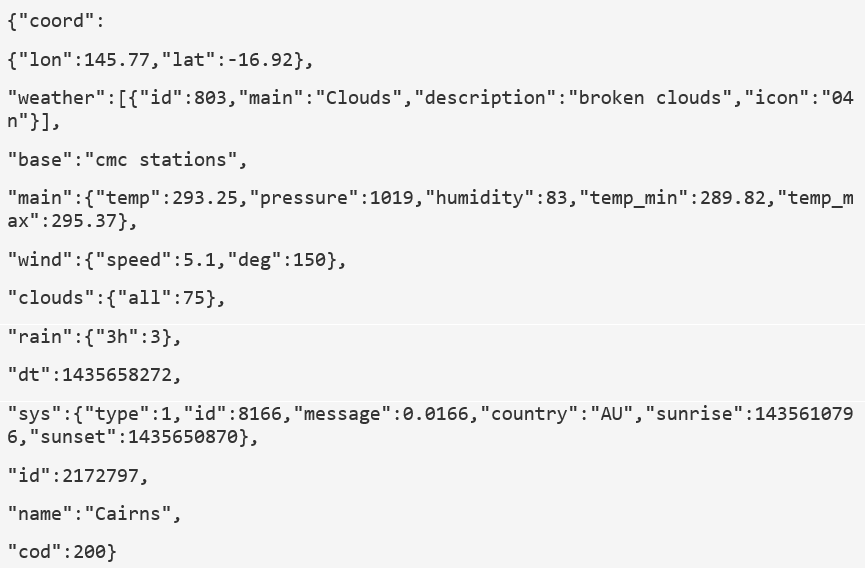
\includegraphics{img_usadas/JSONex.png}
  \caption{Ejemplo de \textit{JSON}}
  \label{fig:json}
\end{figure}


%%%%%%%%%%%%%%%%%%%%%%%%%%%%%%%%%%%%%%%%%%%%%%%%%%%%%%%%%%%%%%%%%%%%%%%%%%%%%%%%
%%%%%%%%%%%%%%%%%%%%%%%%%%%%%%%%%%%%%%%%%%%%%%%%%%%%%%%%%%%%%%%%%%%%%%%%%%%%%%%%
% INSTALACIÓN E IMPLEMENTACIÓN %
%%%%%%%%%%%%%%%%%%%%%%%%%%%%%%%%%%%%%%%%%%%%%%%%%%%%%%%%%%%%%%%%%%%%%%%%%%%%%%%%

\cleardoublepage
\chapter{Instalación e implementación}
En este capítulo se detallan los pasos que hay que realizar para tener configurado un entorno en el que poder hacer este proyecto.

\section{Instalación de componentes necesarios}
\label{sec:instalacion-de-componentes-necesarios}
Para poder realizar este trabajo es necesario tener por un lado todos los paquetes y configuraciones que necesita Liferay, y por otro lado todos los paquetes e instalaciones que necesita React para ser conectado con Liferay. 

\vspace{5mm}
Para utilizar Liferay con React, necesitamos tener un servidor con una versión de Liferay 7.0 o superior, debido a que es la versión a partir de la cual podemos instalar el plugin \textit{JS Portlet Extender}.

En este proyecto se ha descargado el \textit{tomcat} de Liferay 7.1.1\footnote{Descarga tomcat: \url{https://www.liferay.com/es/downloads-community}} . Para poder arrancar el servidor, necesitamos tener una serie de configuraciones e instalaciones que nos permiten utilizar Liferay.

\vspace{5mm}
Lo primero que debemos hacer es descargar es el \textit{JDK} y el \textit{JRE}\footnote{Descarga \textit{JDK} y \textit{JRE}: \url{https://www.oracle.com/technetwork/java/javase/downloads/jdk8-downloads-2133151.html}}  de Java e introducirlos en las variables de entorno del sistema del ordenador de la forma que se muestra en la Figura~\ref{fig:variables-entorno}.
\begin{figure}
  \centering
  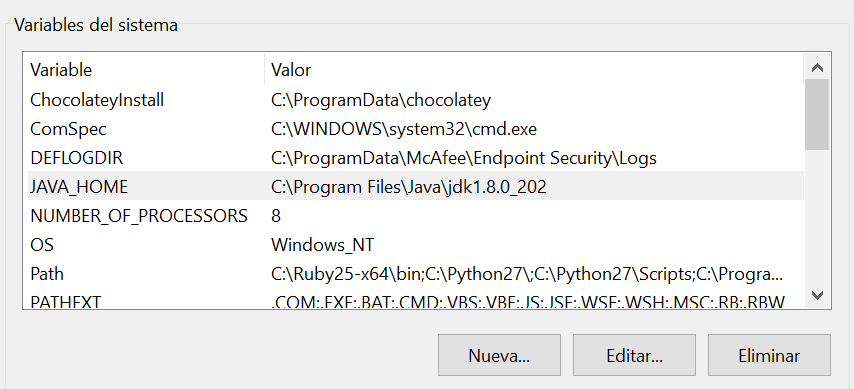
\includegraphics{img_usadas/variablesentornos.png}
  \caption{Ventana de configuración de las variables de entorno}
  \label{fig:variables-entorno}
\end{figure}

\vspace{5mm}
Una vez configuradas las variables de entorno debemos instalar \textit{Node.js}\footnote{Descarga \textit{Node.js}: \url{https://nodejs.org/en/}} , que es necesario para poder utilizar React. \textit{Node.js} es un entorno de ejecución de código abierto para \textit{JavaScript} construido por el motor de \textit{Chrome} y orientado a eventos asíncronos. Proporciona un entorno de ejecución del lado del servidor que compila y ejecuta a velocidades muy altas. Se ejecuta para cada conexión y si no hay conexiones ejecutando \textit{Node.js} no se ejecuta. Esto hace que no haya bloqueos de procesos debido a que no existen los bloqueos, lo que hace que se desarrollen sistemas escalables.

\vspace{5mm}
Con la instalación de \textit{Node.js} obtenemos a la vez el sistema de gestión de paquetes \textit{npm} que es necesario para instalar y manejar las dependencias del proyecto, así como las librerías y los paquetes necesarios. Además de \textit{npm}, necesitamos tener instalado otro manejador de paquetes llamado \textit{Yarn}\footnote{Descarga \textit{Yarn}: \url{https://yarnpkg.com/lang/en/}} , que se caracteriza por tener una velocidad mayor que \textit{npm} debido a que permite descargas en simultaneo.

\vspace{5mm}
Para verificar que tenemos \textit{Node.js}, \textit{npm} y \textit{Yarn} correctamente instalados, es necesario ejecutar en una consola de comandos como en la Figura~\ref{fig:verificacion}.
\begin{figure}
  \centering
  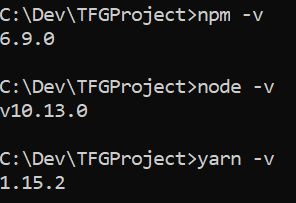
\includegraphics{img_usadas/verificacion.png}
  \caption{Comandos para verificar la instalación de los paquetes}
  \label{fig:verificacion}
\end{figure}

\vspace{20mm}
Con estos pasos, tenemos todas las configuraciones y todos los paquetes necesarios instalados. Ahora es necesario arrancar el servidor de Liferay para tenerlo disponible, si es la primera vez que se ha arrancado, nos aparecerá una ventana de configuración para poder crearnos el usuario y su contraseña, además de poder configurar el idioma del portal. Una vez configurado el usuario y el idioma tendremos un portal disponible con la página principal como se ve en la Figura~\ref{fig:liferay_ini}. Con esto tendremos a disposición todos los componentes y elementos que vienen configurados por defecto con Liferay. Podremos crear páginas y componentes para organizar el portal de la manera deseada.
\begin{figure}[h]
  \centering
  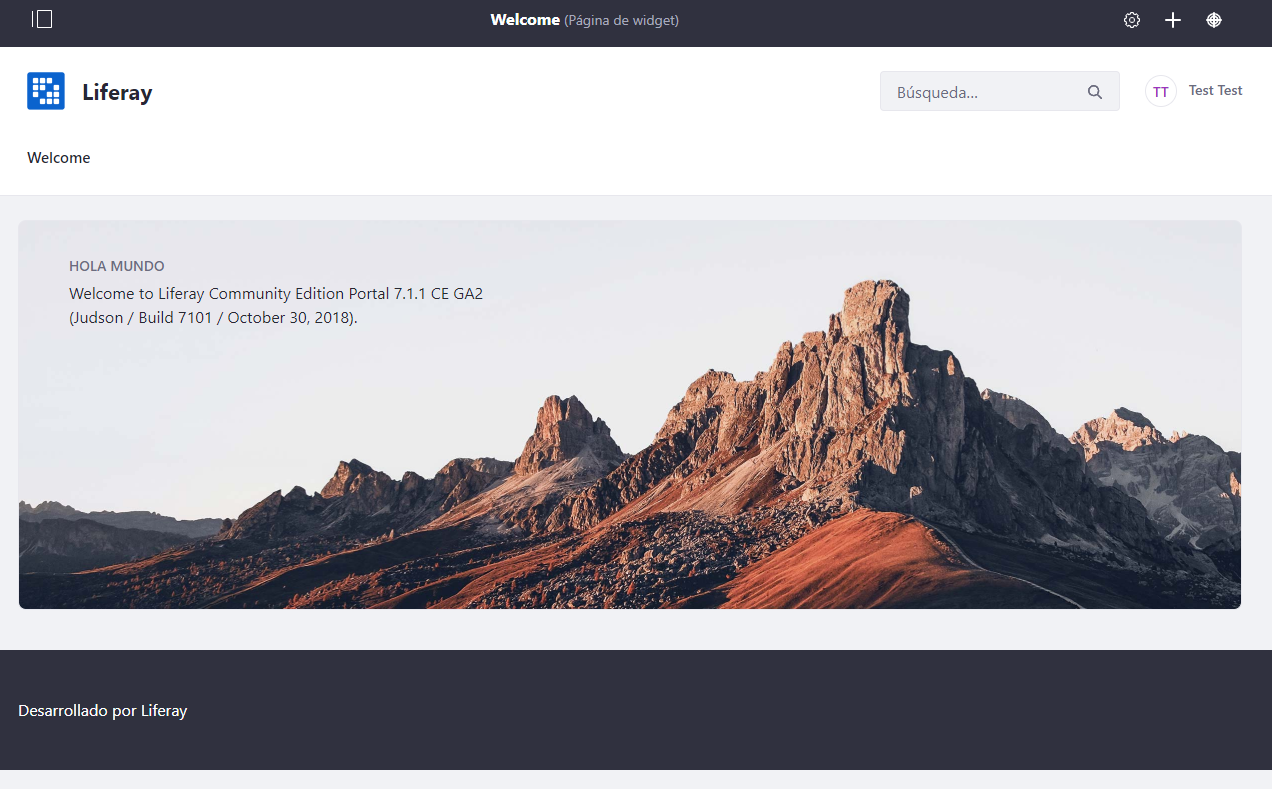
\includegraphics[width=15cm, height=10cm]{img_usadas/liferay_ini.png}
  \caption{Visualización inicial de la página principal del portal de Liferay}
  \label{fig:liferay_ini}
\end{figure}


\section{Creación portlet React}
\label{sec:creacion-portlet-react}
Una vez tenemos un servidor Liferay arrancado y en funcionamiento, podemos empezar a integrar React con Liferay. Para ello es necesario instalar un generador de \textit{Yeoman}\footnote{\url{https://yeoman.io/}}, la instalación se realiza con el siguiente comando: 
\begin{verbatim}
    npm install -g yo
\end{verbatim}

Con el generador de \textit{Yeoman} instalado, el siguiente paso es instalar el generador de los paquetes de Liferay (liferay-bundle) de la siguiente manera:
\begin{verbatim}
    npm install generator-liferay-bundle
\end{verbatim}

Con ambos generadores instalados, ya podemos crear el portlet de React con el comando 
\begin{verbatim}
    yo liferay-bundle
\end{verbatim} 
que nos permite elegir el tipo de proyecto que queremos crear como se muestra en la Figura~\ref{fig:liferay_type}.
\begin{figure}[h]
  \centering
  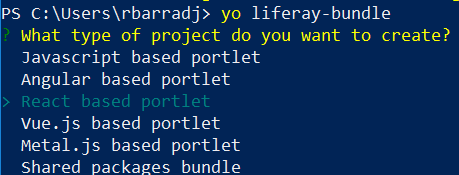
\includegraphics{img_usadas/liferay-bundle-react.png}
  \caption{Elección del tipo de proyecto}
  \label{fig:liferay_type}
\end{figure}

El tipo de proyecto que queremos crear en este caso es "\textit{React based portlet}", al elegirlo debemos configurar las opciones que se muestran en la Figura~\ref{fig:liferay_generator_portlet}.
\begin{figure}[t]
  \centering
  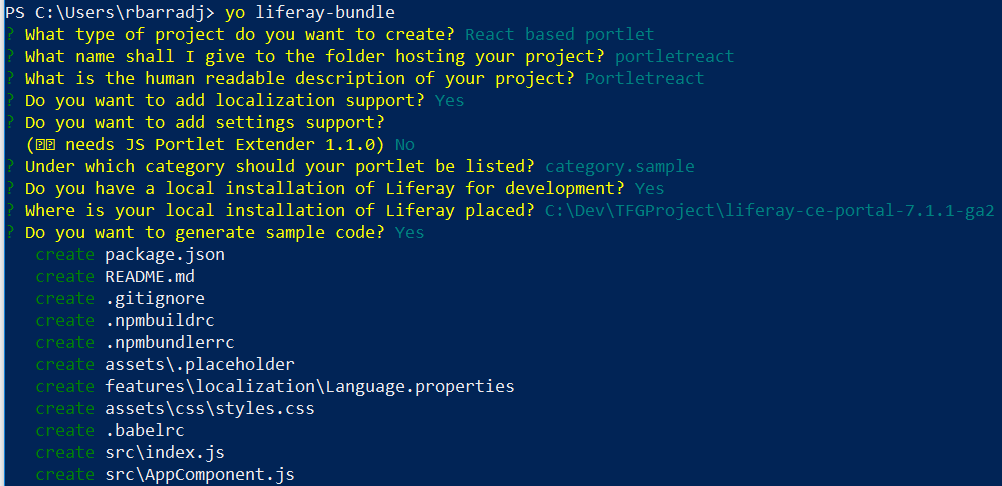
\includegraphics{img_usadas/liferay-bundle-generator.png}
  \caption{Creación portlet React}
  \label{fig:liferay_generator_portlet}
\end{figure}

En dicha Figura~\ref{fig:liferay_generator_portlet} podemos ver que al crear el proyecto debemos darle el nombre que queramos, en este caso "portletreact", la descripción del proyecto y la categoría en la que queremos que aparezca en el portal de Liferay, en este caso "\textit{Ejemplo}". 
Además, nos pregunta si tenemos alguna instalación local de Liferay, que es la que hemos realizado anteriormente, al decirle "\textit{Yes}" nos pregunta sobre la localización de dicha instalación, donde debemos poner la ruta en la que está el \textit{tomcat} instalado en el apartado~\ref{sec:instalacion-de-componentes-necesarios}.

Al generar un código de ejemplo, se generan los paquetes que vemos en la Figura~\ref{fig:liferay_generator_portlet} que nos permiten la conectividad entre React y Liferay. Por medio del fichero "\textit{package.json}" se declaran las dependencias del portlet como se puede ver en la Figura~\ref{fig:package_ini}. En el fichero "\textit{index.js}" se reciben los campos "\textit{contextPath}", que es la ruta del contexto donde se bajan los recursos estáticos del portlet, y "\textit{portletElementId}", que es el identificador del nodo que permite la conectividad con el framework para generar la interfaz de usuario.
\begin{figure}[h]
  \centering
  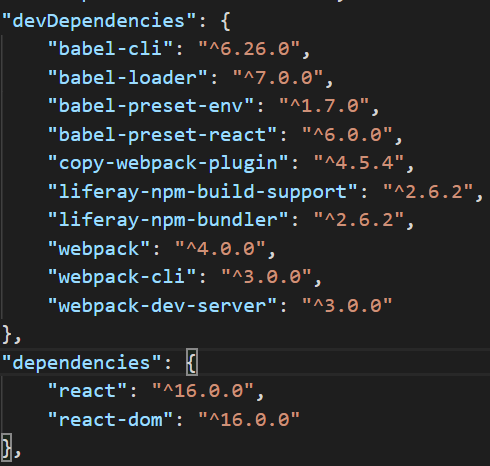
\includegraphics[width=8cm, height=6cm]{img_usadas/package_ini.png}
  \caption{Visualización del fichero "\textit{package.json}"}
  \label{fig:package_ini}
\end{figure}


\vspace{5mm}
\section{Desarrollo de la aplicación} 
\label{sec:desarrollo-aplicacion}
Una vez hemos creado el portlet y tenemos todos los paquetes necesarios instalados, es hora de comenzar a desarrollar la aplicación. En este apartado se van a explicar las configuraciones iniciales necesarias para poder usar las librerías que permiten la generación de los gráficos, y las principales funciones utilizadas para obtener los datos que se van a mostrar.

\vspace{5mm}
El primer paso para desarrollar la aplicación es instalar las librerías que nos permiten desarrollar la aplicación utilizando React. Para instalar las librerías, recomiendo utilizar la herramienta \textit{Yarn}, comentada en el apartado~\ref{sec:instalacion-de-componentes-necesarios}, debido a que no da conflictos con las dependencias ya instaladas, por el contrario, si usamos \textit{npm} podemos llegar a tener algún tipo de conflicto.

Las primeras librerías que debemos instalar son las que nos permiten programar utilizando \textit{ECMAScript}. Se instalan con los siguientes comandos: 
\begin{verbatim}
    yarn add eslint
    yarn add babel-preset-es2015
    yarn add babel-plugin-transform-class-properties
\end{verbatim} 
Para verificar que se han instalado bien las librerías, comprobamos que se han añadido al fichero \textit{"package.json"} tal y como se muestra en la Figura~\ref{fig:package_babelrc}.
\begin{figure}[h]
  \centering
  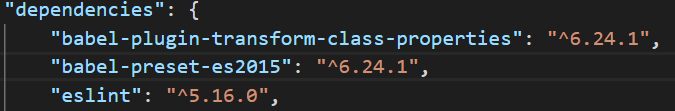
\includegraphics{img_usadas/package_babelrc.png}
  \caption{Visualización de las librerías de \textit{ECMAScript} en el fichero \textit{"package.json"}}
  \label{fig:package_babelrc}
\end{figure}

Una vez las librerías están instaladas, debemos modificar el fichero "\textit{.babelrc}" de la siguiente manera:
\begin{verbatim}
    {
	        "presets": ["es2015", "react"],
	        "plugins": ["transform-class-properties"]
    }
\end{verbatim}

Con estas configuraciones ya se puede empezar a programar con React. El siguiente paso es instalar las librerías necesarias para generar los gráficos y transformar los datos recogidos de la \textit{API}. Estas librerías son "\textit{react-chartjs-2"}, "\textit{react-chartjs2"} y "\textit{chart.js"}. Se instalan usando los siguientes comandos: 
\begin{verbatim}
    yarn add react-chartjs-2
    yarn add react-chartjs2
    yarn add chart.js
\end{verbatim} 
Para verificar que se han instalado bien las librerías, comprobamos que se han añadido al fichero \textit{"package.json"} tal y como se muestra en la Figura~\ref{fig:package_chart}.
\begin{figure}[h]
  \centering
  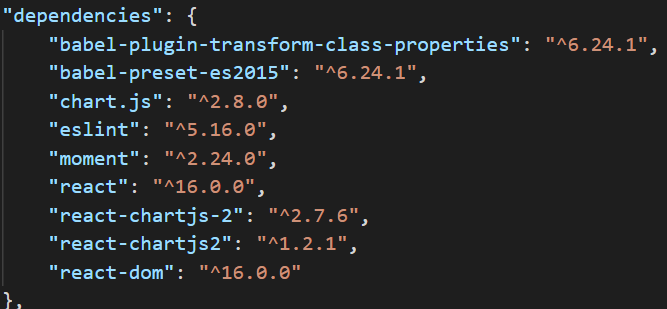
\includegraphics{img_usadas/package_chart.png}
  \caption{Visualización de las librerías en el fichero \textit{"package.json"}}
  \label{fig:package_chart}
\end{figure}

Como podemos ver, con estas librerías ya se puede empezar a generar gráficos. El siguiente paso es obtener los datos de la \textit{API}. 

En este proyecto se ha utilizado la \textit{API OpenWeatherMap}\footnote{\url{https://openweathermap.org/}}, en la cual podemos obtener los datos meteorológicos para el día actual, y los datos meteorológicos de una semana.
Estos datos vienen en formato \textit{JSON}.

\vspace{5mm}
Para transformar estos datos en legibles, ha sido necesario emplear la librería "\textit{moment}", instalada con el siguiente comando: 
\begin{verbatim}
    yarn add moment
\end{verbatim} 

Para la transformación de los datos meteorológicos, se ha usado una función como se muestra en la Figura~\ref{fig:transform_day}.
\begin{figure}[h]
  \centering
  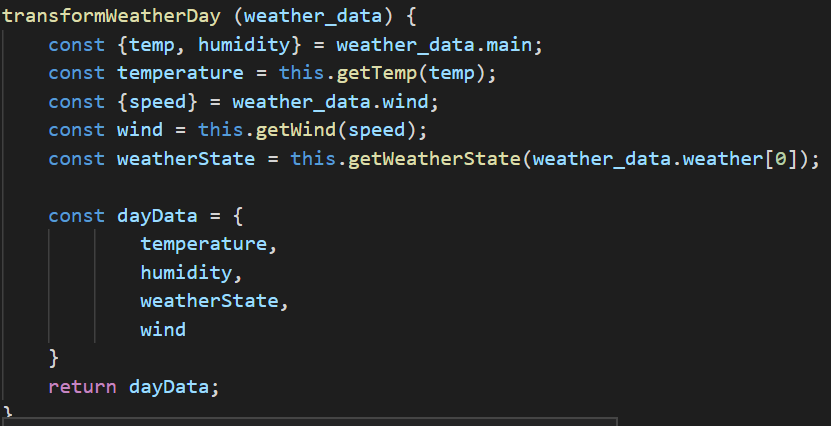
\includegraphics[width=12cm, height=5cm]{img_usadas/transform_day.png}
  \caption{Función para transformar los datos del \textit{JSON}}
  \label{fig:transform_day}
\end{figure}

\vspace{5mm}
Para la transformación de las horas del día se ha usado otra función, en la cual se ha usado la librería \textit{"moment"}, como podemos ver en la Figura~\ref{fig:transform_data}.
\begin{figure}[h]
  \centering
  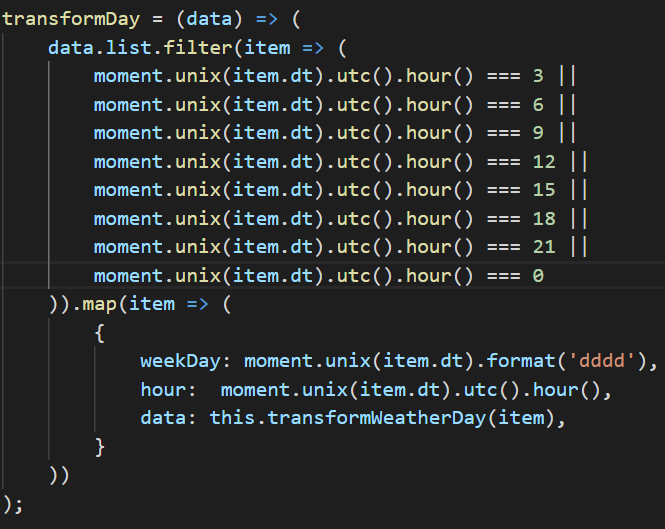
\includegraphics[width=10cm, height=6cm]{img_usadas/transform_data.png}
  \caption{Función para transformar las horas del \textit{JSON}}
  \label{fig:transform_data}
\end{figure}

Una vez obtenemos los datos legibles, ya podemos empezar a usarlos y a generar los gráficos con ellos. Estos gráficos se verán en el Capítulo~\ref{chap:resultados_obtenidos}.


\section{Despliegue en Liferay} 
\label{sec:despliegue-liferay}
Tras realizar el desarrollo del portlet, es hora de desplegarlo y construirlo en el portal de Liferay, para ello debemos tener el servidor arrancado. Antes de desplegarlo hay que construirlo, ejecutando el siguiente comando, en la ruta en la que tenemos guardado el proyecto:
\begin{verbatim}
    npm run build
\end{verbatim} 
Este comando construye las rutas que hay en el proyecto y construye las dependencias que haya en el "\textit{package.json}". La ejecución del comando se puede ver en la Figura~\ref{fig:npm_build}.
\begin{figure}[h]
  \centering
  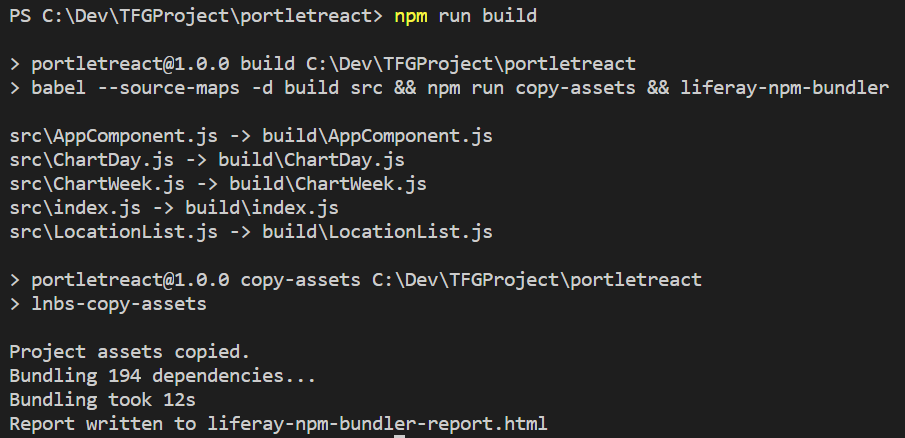
\includegraphics[width=12cm, height=5cm]{img_usadas/npm_build.png}
  \caption{Ejecución del comando \textit{"build"}}
  \label{fig:npm_build}
\end{figure}

Tras construir las dependencias y las rutas del proyecto, hay que desplegar el proyecto en Liferay con el siguiente comando: 
\begin{verbatim}
    npm run deploy
\end{verbatim}
Este comando realiza el despliegue del portlet a Liferay, su ejecución se muestra en la Figura~\ref{fig:deploy}.
\begin{figure}[h]
  \centering
  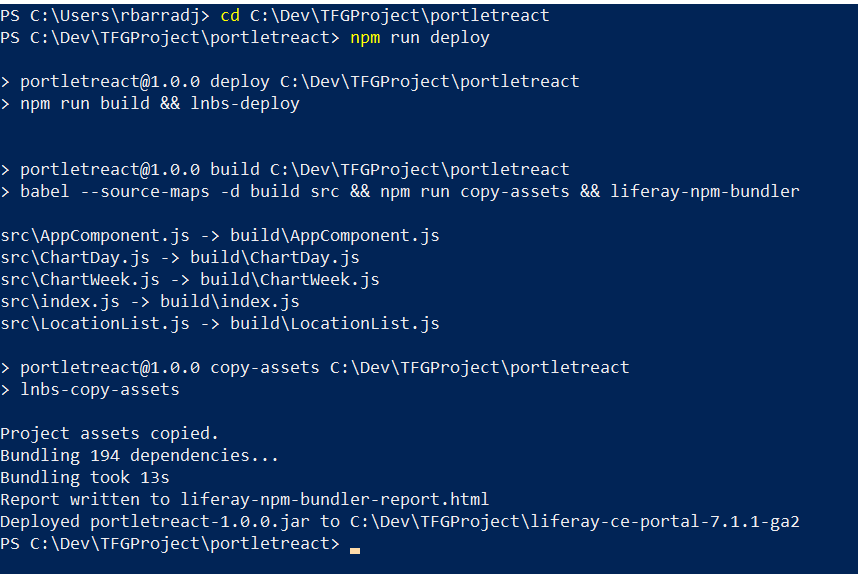
\includegraphics[width=11cm, height=8cm]{img_usadas/deploy.png}
  \caption{Ejecución del comando \textit{"deploy"}}
  \label{fig:deploy}
\end{figure}

Como podemos ver, al hacer "\textit{deploy}" se hace lo mismo que en "\textit{build"}, añadiendo el despliegue al \textit{tomcat} configurado en el apartado~\ref{sec:creacion-portlet-react} donde introducimos la ruta en la que lo teníamos.

\vspace{5mm}
Con el servidor arrancado, una vez se completa el despliegue, en la consola deberá aparecer el mensaje que se ve en la Figura~\ref{fig:started}.
\begin{figure}[h]
  \centering
  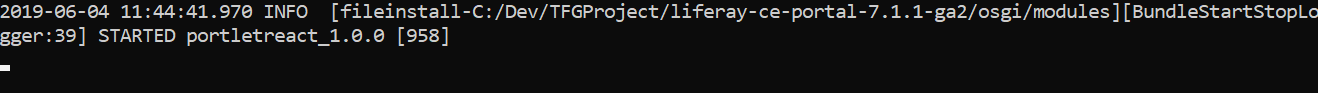
\includegraphics[width=15cm]{img_usadas/started.png}
  \caption{Visualización de la consola del servidor al desplegar}
  \label{fig:started}
\end{figure}

\vspace{5mm}
Una vez vemos el mensaje "STARTED" dentro de la consola, el portlet estará disponible en el portal de Liferay, en la categoría que introdujimos en el apartado~\ref{sec:creacion-portlet-react}. En este caso, la categoría es "\textit{Ejemplo}", por lo que, una vez logueados, seleccionamos la categoría en la sección de configuración de los contenidos de Liferay y arrastramos el portlet, de la forma que vemos en la Figura~\ref{fig:liferay_ex}.
\begin{figure}[h]
  \centering
  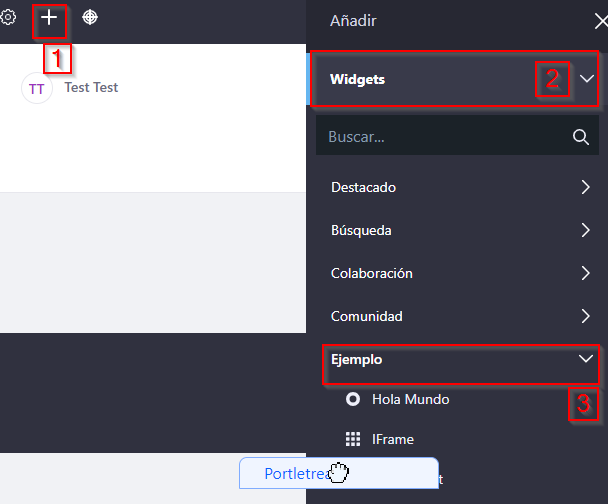
\includegraphics{img_usadas/liferay_ex.png}
  \caption{Despliegue del portlet en Liferay}
  \label{fig:liferay_ex}
\end{figure}

\vspace{5mm}
Posicionamos el componente en la zona que queramos del portal y tendríamos el portlet listo para visualizarse de la forma que veremos en el Capítulo~\ref{chap:resultados_obtenidos}.



%%%%%%%%%%%%%%%%%%%%%%%%%%%%%%%%%%%%%%%%%%%%%%%%%%%%%%%%%%%%%%%%%%%%%%%%%%%%%%%%
%%%%%%%%%%%%%%%%%%%%%%%%%%%%%%%%%%%%%%%%%%%%%%%%%%%%%%%%%%%%%%%%%%%%%%%%%%%%%%%%
% RESULTADOS %
%%%%%%%%%%%%%%%%%%%%%%%%%%%%%%%%%%%%%%%%%%%%%%%%%%%%%%%%%%%%%%%%%%%%%%%%%%%%%%%%

\cleardoublepage
\chapter{Resultados obtenidos}
\label{chap:resultados_obtenidos}
Una vez se ha desplegado el portlet en Liferay y se ha movido a la zona donde se desea, podemos empezar a usar el componente. En este capítulo se van a detallar los resultados obtenidos al desarrollar e integrar la aplicación.


\section{Visualización inicial}
\label{sec:visualizacion-inicial}
La visualización inicial del portlet es la que se ve en la Figura~\ref{fig:pantalla_ini}, donde vemos una breve descripción del funcionamiento del componente, un selector para seleccionar una ciudad y un mensaje indicando que debemos elegir una ciudad.
\begin{figure}[h]
  \centering
  
\includegraphics[width=15cm]{img_usadas/pantalla_ini.png}
  \caption{Visualización inicial del portlet}
  \label{fig:pantalla_ini}
\end{figure}

\vspace{5mm}
Si desplegamos el selector veremos una lista de ciudades, como se muestra en la Figura~\ref{fig:seleccion_ciudad}, en la cual debemos seleccionar una ciudad para mostrar sus datos, tal y como se verá en los siguientes apartados de este capítulo.
\begin{figure}[h]
  \centering
  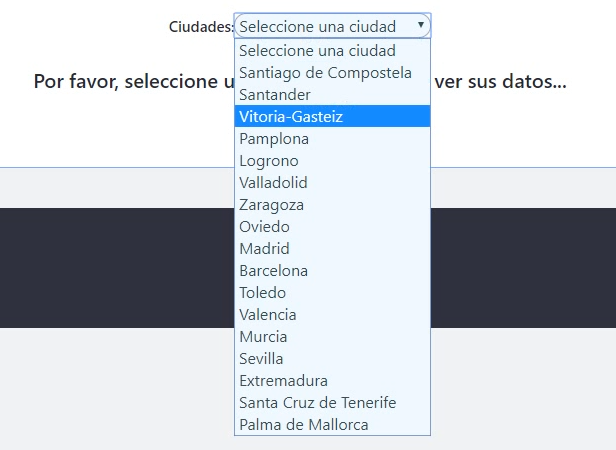
\includegraphics{img_usadas/seleccion_ciudad.png}
  \caption{Visualización del selector de las ciudades}
  \label{fig:seleccion_ciudad}
\end{figure}



\section{Visualización datos diarios}
\label{sec:visualizacion-diaria}
Al seleccionar la ciudad, se cargarán los gráficos con los datos diarios por defecto, como se ve en la Figura~\ref{fig:pantalla_diaria}. En dicha imagen se pueden ver los datos de la temperatura, la humedad y el viento a unas determinadas horas del día. Estos datos nos los proporciona la \textit{API} de 3 horas en 3 horas, de ahí que se muestren en los gráficos los datos cada 3 horas.
\begin{figure}[h]
  \centering
  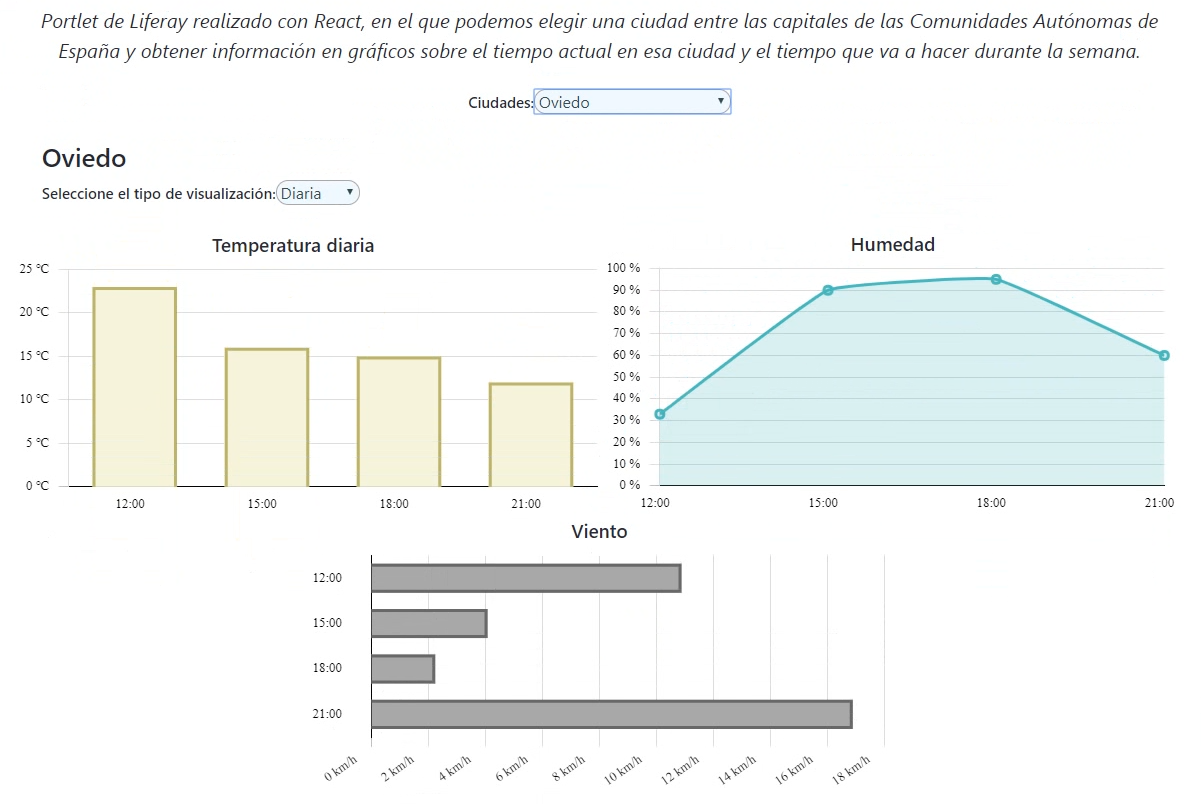
\includegraphics[width=13cm, height=7cm]{img_usadas/pantalla_diaria.png}
  \caption{Visualización de los gráficos para los datos diarios}
  \label{fig:pantalla_diaria}
\end{figure}

\vspace{5mm}
Para la temperatura diaria, se muestran los datos cada 3 horas en \textit{ºC}, para la humedad se muestra el porcentaje de humedad en esas horas, y para el viento se muestran los datos en \textit{km/h}.

\vspace{5mm}
Si nos posicionamos sobre alguna barra de algún gráfico, se verá información detallada sobre la hora en la que nos hemos posicionado, tal y como se muestra en la Figura~\ref{fig:detalle_chart}.
\begin{figure}[h]
  \centering
  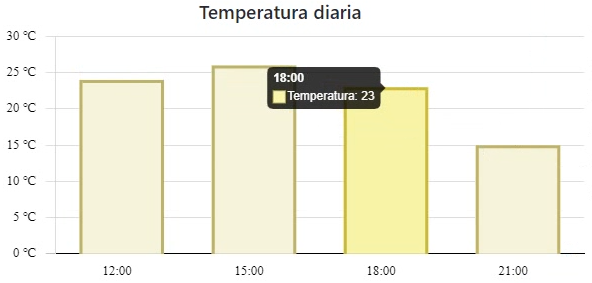
\includegraphics{img_usadas/detalle_chart.png}
  \caption{Visualización en detalle del gráfico}
  \label{fig:detalle_chart}
\end{figure}

En este caso, se ve información de la temperatura exacta a las 18:00. Si nos posicionáramos sobre otro tipo de gráfico, veríamos información detallada de la humedad exacta o del viento exacto en ese momento.
Si se quiere cambiar la ciudad, se podría seleccionar otro ciudad y se cargarían los nuevos datos para la ciudad seleccionada.

\vspace{5mm}
En esta misma pantalla, hay un selector que permite seleccionar el tipo de visualización, como se ve en la Figura~\ref{fig:seleccion_tipo}, eligiendo entre visualización diaria, como se ve en este apartado, o eligiendo visualización semanal, como se verá en el apartado~\ref{sec:visualizacion-semanal}.
Si seleccionamos en el desplegable el tipo de visualización diferente a la visualización de la pantalla en la que nos encontramos, la página se carga y se muestran los datos del tipo seleccionado.
\begin{figure}[h]
  \centering
  
\includegraphics{img_usadas/seleccion_tipo.png}
  \caption{Selector para el elegir el tipo de visualización}
  \label{fig:seleccion_tipo}
\end{figure}


\section{Visualización temperatura semanal}
\label{sec:visualizacion-semanal}
Al seleccionar en el desplegable "Semanal", se cargan los datos para mostrarse el gráfico de la tempetatura semanal en una ciudad, tal y como se ve en la Figura~\ref{fig:pantalla_semanal}.
\begin{figure}[h]
  \centering
  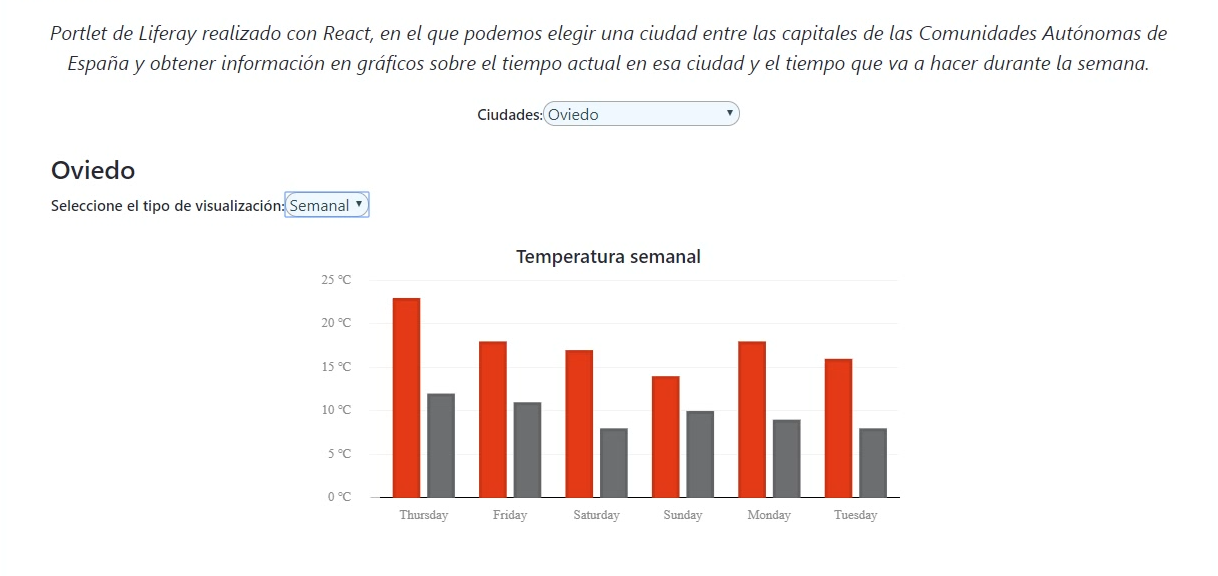
\includegraphics[width=13cm, height=7cm]{img_usadas/pantalla_semanal.png}
  \caption{Visualización del gráfico para los datos semanales}
  \label{fig:pantalla_semanal}
\end{figure}

En esta imagen se ven las temperaturas máximas, en rojo, y mínimas, en gris, que hay en la semana. De igual manera que pasa con los gráficos diarios, si pasamos por encima de alguna barra del gráfico se verá información detallada sobre dicha barra, indicando el día y la temperatura.

\vspace{5mm}
Desde esta visualización se puede ir a la visualización diaria, seleccionando en el desplegable del tipo de visualización la opción "Diaria". También se puede cambiar la ciudad para poder comparar las temperaturas de distintas ciudades.




%%%%%%%%%%%%%%%%%%%%%%%%%%%%%%%%%%%%%%%%%%%%%%%%%%%%%%%%%%%%%%%%%%%%%%%%%%%%%%%%
%%%%%%%%%%%%%%%%%%%%%%%%%%%%%%%%%%%%%%%%%%%%%%%%%%%%%%%%%%%%%%%%%%%%%%%%%%%%%%%%
% CONCLUSIONES %
%%%%%%%%%%%%%%%%%%%%%%%%%%%%%%%%%%%%%%%%%%%%%%%%%%%%%%%%%%%%%%%%%%%%%%%%%%%%%%%%

\cleardoublepage
\chapter{Conclusiones}
\label{chap:conclusiones}
En este último capítulo, se va a realizar un análisis de los resultados obtenidos en base a los objetivos planteados, de la aplicación de los conocimientos aprendidos y de los posibles trabajos futuros relacionados con este proyecto.

\section{Consecución de los objetivos}
\label{sec:consecucion_objectivos}
Si volvemos a los objetivos marcados para este proyecto, el objetivo principal era integrar React con Liferay, pudiendo utilizar sus bibliotecas y tener una aplicación de React dentro de Liferay para poder gestionarla de la manera que queramos. Este objetivo se ha cumplido como hemos podido ver en el desarrollo de este trabajo, pudiendo añadir y eliminar dependencias para crear la conexión entre Liferay y React, y pudiendo usar las bibliotecas de React dentro de la plataforma de Liferay.

\vspace{5mm}
Los objetivos secundarios eran objetivos de formación y familiarización con las tecnologías utilizadas. Este objetivo, por mi parte, también se ha cumplido, debido a que eran tecnologías que no había usado nunca y he podido defenderme con ellas y al final he podido conectarlas. He aprendido el manejo de las dependencias de Liferay y la navegación entre la plataforma, permitiendo diseñar portales a mi gusto, así como el manejo con las funciones y métodos de React y JavaScript, algo que considero muy importante viendo el mercado laboral que hay actualmente.

\section{Aplicación de lo aprendido}
\label{sec:consecucion_objectivos}
Los conocimientos aprendidos me han servido para ser más independiente en la empresa en la que estoy trabajando, debido a que he aprendido a entender el comportamiento de Liferay con los portlets, algo que es muy importante a la hora de crear páginas web utilizando este gestor de contenidos.

\vspace{5mm}
Además me ha servido para poder enseñar a mis compañeros a añadir portlets realizados con bibliotecas de React, algo que no se había hecho en la empresa de la manera que se ha hecho en este proyecto. 

Incluir librerías de JavaScript en Liferay de esta manera, ejecutando comandos y desarrollando en JavaScript el código de la aplicación, hace que el desarrollo sea más rápido y se puedan realizar más pruebas sobre la aplicación, debido a que podemos ir probando la aplicación de JavaScript sin necesidad de desplegar en Liferay.

Esto es algo importante, ya que una vez estás realizando algún tipo de componente, para probarlo en Liferay hay que desplegar cada cambio que se haga y así poder visualizarlo, mientras que si empleamos JavaScript, podemos ver los cambios simplemente con guardar el código.

 
\section{Trabajos futuros}
\label{sec:trabajos_futuros}
En este proyecto, se ha integrado React con Liferay, haciendo que el código programado en React se comunique y se visualice en Liferay.

Un posible trabajo futuro sería poder comunicar Liferay con React, no React con Liferay como se ha hecho en este trabajo. Esto es, que se pueda realizar un portlet con React, que al estar en Liferay, se pueda configurar desde la configuración de Liferay, para comunicarle dichas configuraciones a React, y se desarrolle el portlet según se configure.

En este caso, se podría haber realizado una configuración en el portlet de Liferay para poder elegir el color de los gráficos, o la forma en la que queremos que se visualicen los gráficos. Estas configuraciones realizadas desde el componente en Liferay podrían haber cambiado dichos colores o dichas formas.

\vspace{5mm}
Otro posible trabajo futuro sería poder incluir \textit{Redux}\footnote{\url{https://es.redux.js.org/}}, que hace que se actualice automáticamente la aplicación si un componente cambia, lo que permite que se individualicen los problemas de una manera más rápida. Si tenemos una aplicación muy grande y se realiza un cambio en un componente una vez el proyecto está casi acabado, \textit{Redux} hace que se actualice el cambio en la aplicación, al igual que sus variables sin necesidad de hacerlo manualmente.

Otra ventaja de \textit{Redux} es que si se actualiza el estado de una variable en un componente, se actualiza también en el resto de componentes del programa.


%%%%%%%%%%%%%%%%%%%%%%%%%%%%%%%%%%%%%%%%%%%%%%%%%%%%%%%%%%%%%%%%%%%%%%%%%%%%%%%%
%%%%%%%%%%%%%%%%%%%%%%%%%%%%%%%%%%%%%%%%%%%%%%%%%%%%%%%%%%%%%%%%%%%%%%%%%%%%%%%%
% APÉNDICE(S) %
%%%%%%%%%%%%%%%%%%%%%%%%%%%%%%%%%%%%%%%%%%%%%%%%%%%%%%%%%%%%%%%%%%%%%%%%%%%%%%%%

\cleardoublepage
\appendix



%%%%%%%%%%%%%%%%%%%%%%%%%%%%%%%%%%%%%%%%%%%%%%%%%%%%%%%%%%%%%%%%%%%%%%%%%%%%%%%%
%%%%%%%%%%%%%%%%%%%%%%%%%%%%%%%%%%%%%%%%%%%%%%%%%%%%%%%%%%%%%%%%%%%%%%%%%%%%%%%%
% BIBLIOGRAFIA %
%%%%%%%%%%%%%%%%%%%%%%%%%%%%%%%%%%%%%%%%%%%%%%%%%%%%%%%%%%%%%%%%%%%%%%%%%%%%%%%%

\cleardoublepage

% Las siguientes dos instrucciones es todo lo que necesitas
% para incluir las citas en la memoria
\bibliographystyle{abbrv}
\bibliography{memoria}
% Alternativa: haciendo referencia a memoria.bib -> \bibliography{memoria}  % memoria.bib es el nombre del fichero que contiene
% las referencias bibliogr�ficas. Abre ese fichero y mira el formato que tiene,
% que se conoce como BibTeX. Hay muchos sitios que exportan referencias en
% formato BibTeX. Prueba a buscar en http://scholar.google.com por referencias
% y ver�s que lo puedes hacer de manera sencilla.
% M�s informaci�n: 
% http://texblog.org/2014/04/22/using-google-scholar-to-download-bibtex-citations/


\end{document}